% intro

Real-time Transport Protocol (RTP)~\cite{rfc3550} is suitable for multimedia
telephony (voice-over-IP, video conferencing, telepresence systems),
multimedia streaming (video-on-demand, live streaming), and multimedia
broadcast. RTP's design is based on the fundamental principles of \textit
{application-layer framing} and \textit{integrated layer
processing}~\cite{clark:alf}, i.e., it provides the following mechanisms:
source identification, packet playout time, packet loss and reordering, report
packet delay variation (jitter), and payload type identification.

The `synchronisation source' (SSRC) assists in determining the source
endpoint, typically useful when an endpoint sends multiple media streams that
need to be synchronized (e.g., Audio/Video lip-sync). The `RTP timestamp'
assists in playing out the received packets at the appropriate instance of
time and recomposing the media frame from RTP packets. The `RTP sequence
number' assists in identifying the lost packets and re-ordering packets in
case of out-of-order packet arrival. Lastly, RTP uses `payload formats' to
describe the encoding of the media data it is carrying. Consequentely, each
codec needs to specify its corresponding payload format. (See
Figure~\ref{fig:3:rtp.hdr} for packet header format)

\begin{figure}[!htbp]
\centerline{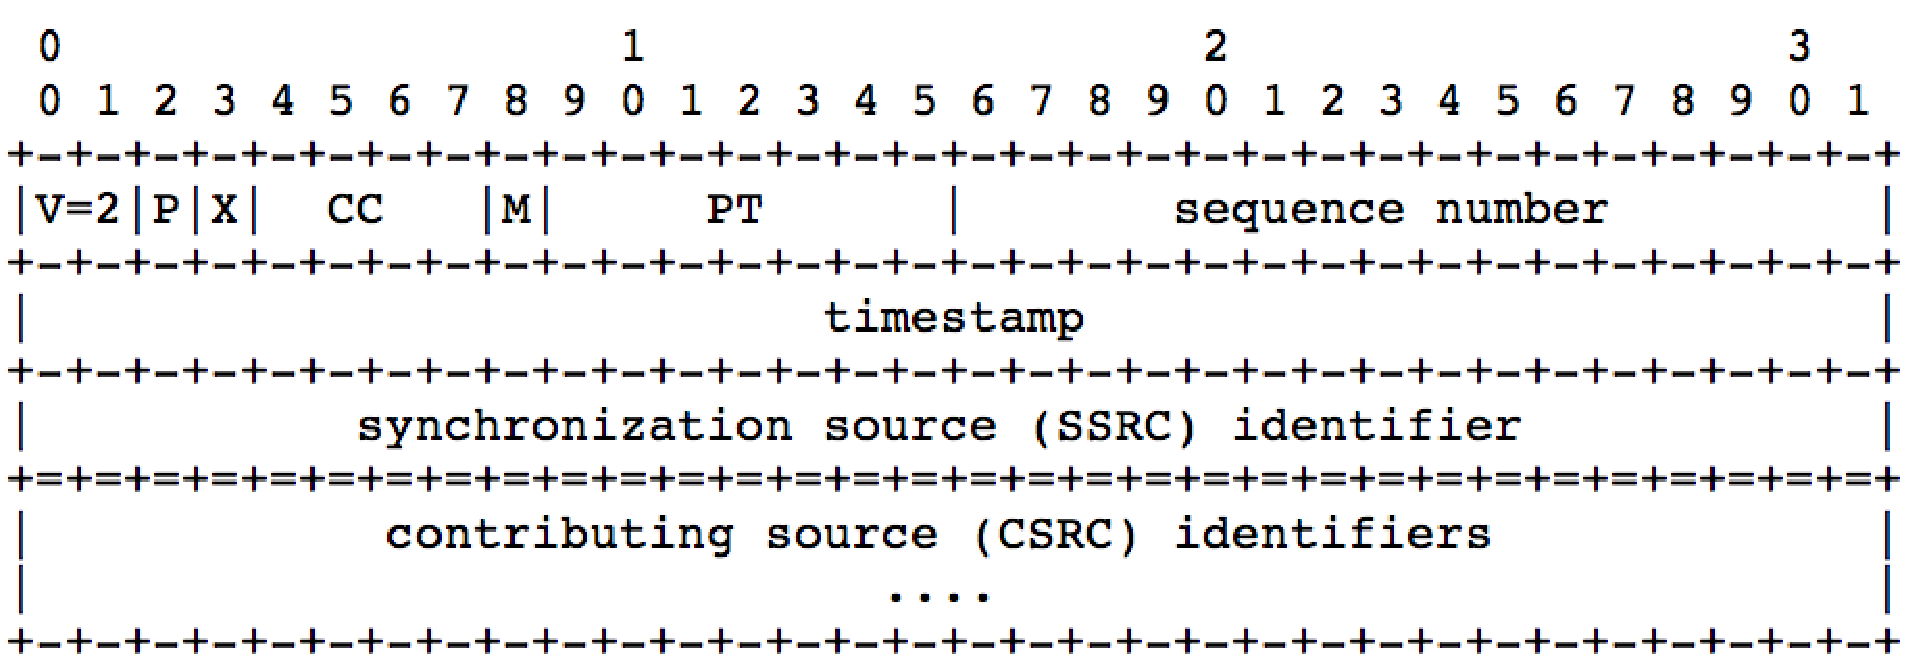
\includegraphics[width=\columnwidth]{fig_hdr_rtp}}
\caption{RTP header}
\label{fig:3:rtp.hdr}
\end{figure}

RTP utilizes RTP Control Protocol (RTCP) to monitor the performance of the
media stream. Using RTCP reports, the endpoints report loss fraction, jitter,
highest sequence number received, and calculate RTT. The RTCP reports also
assist in synchronizing the media streams (audio and video) by relating the
RTP timestamps of the individual media streams to the wall clock time and
measuring RTT. (See Figure~\ref{fig:3:rtcp.hdr} for packet header format)

\begin{figure}
\centerline{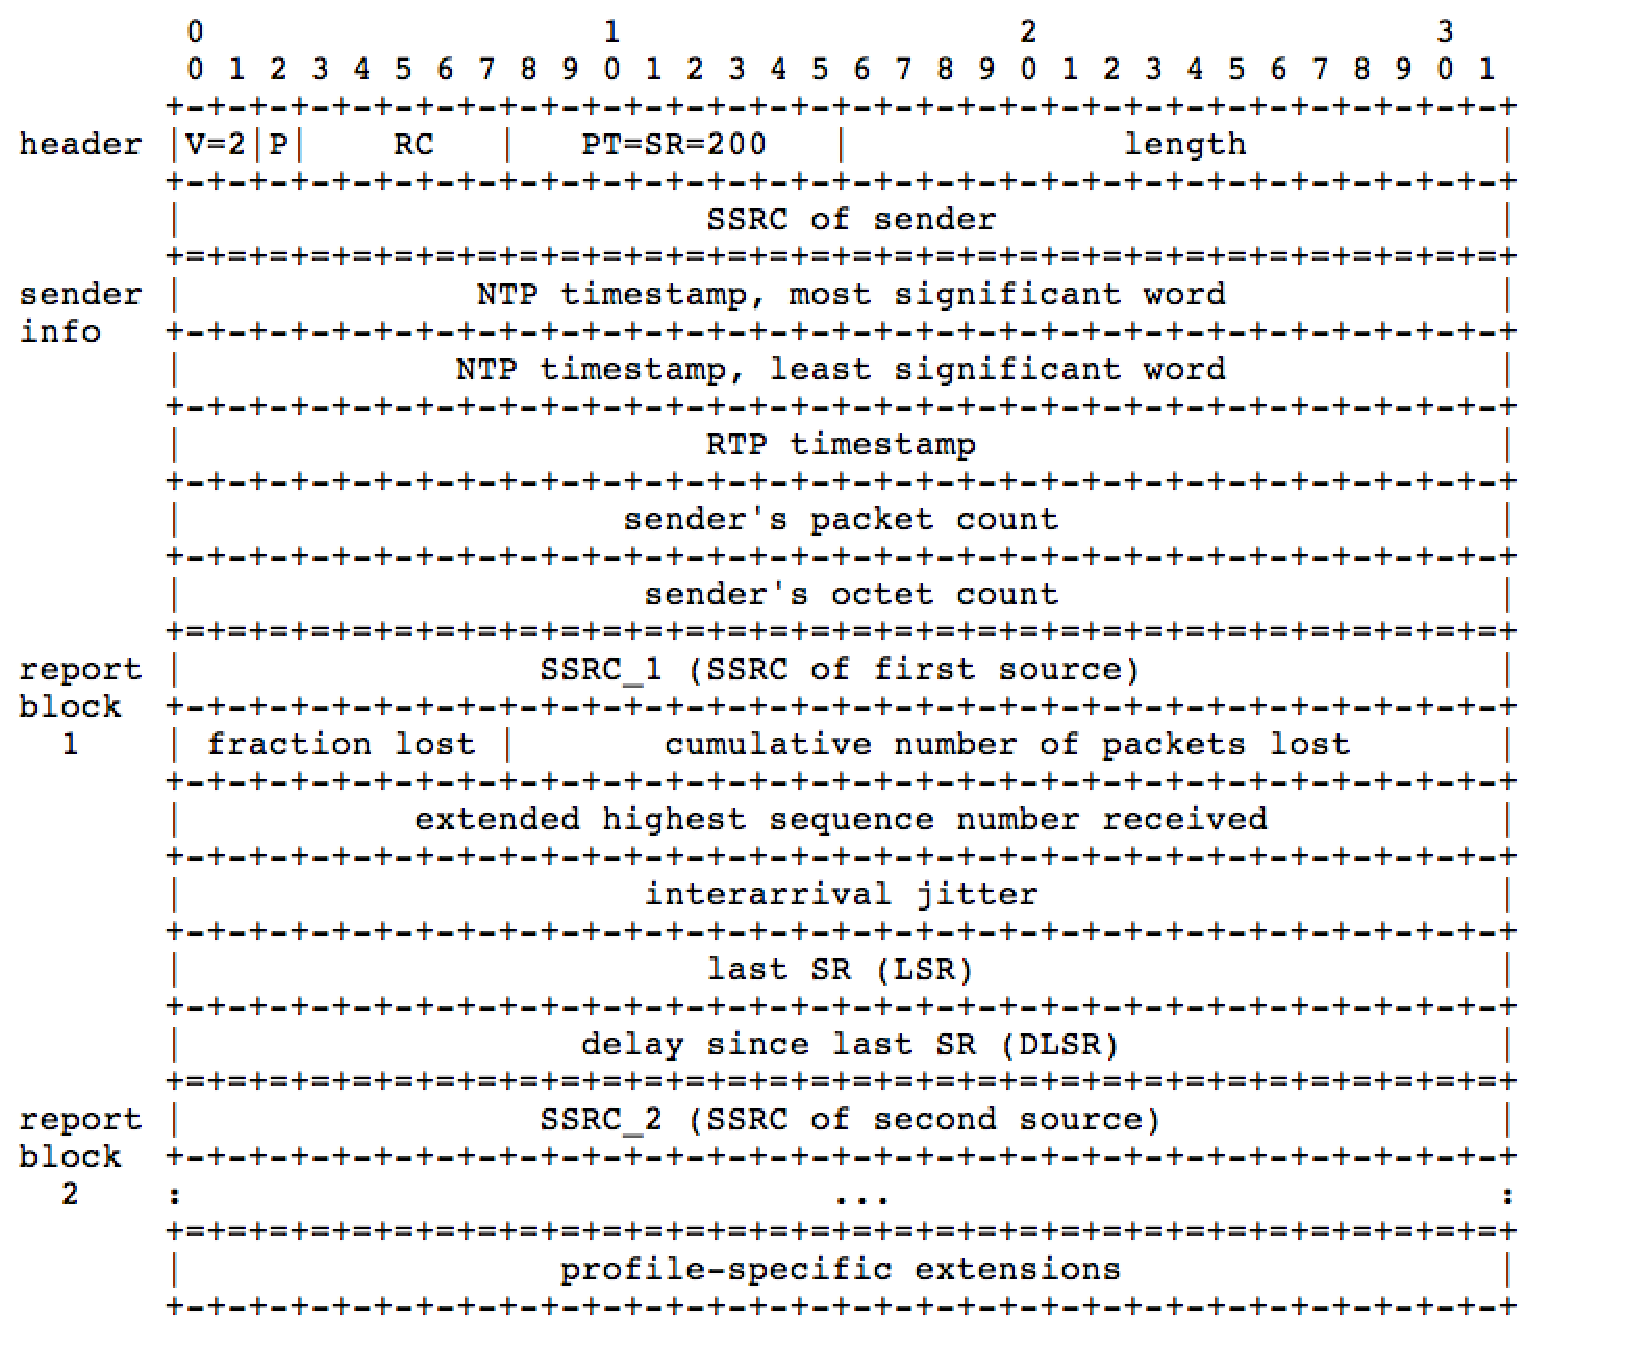
\includegraphics[width=\columnwidth]{fig_hdr_rtcp}}
\caption{RTCP header}
\label{fig:3:rtcp.hdr}
\end{figure}

\section{RTCP Internval}
% timing

A closed control loop is formed by sending RTP media packets and receiving
RTCP feedback packets. Unlike TCP, RTCP feedback interval is not associated to
the path's RTT and RTCP packets are sent periodically. To ensure that the RTCP
reports are not sent too frequently, the endpoints limit the feedback rate to
$5\%$ of the \textit{media rate}, typically, the RTCP interval is set to $5
\pm 2.5$~s. However, the slow control loop can cause instability and
oscillation in the media bit rate.


% avpf

\section{Codec Control}
% codec control

% relationship with SDP
\section{RTP Extensions}
\label{rtp.ext}
